% Copyright 2015-2016 Dan Foreman-Mackey and the co-authors listed below.

\documentclass[manuscript, letterpaper]{aastex6}

\pdfoutput=1

\include{vc}
% Automatically generated
\newcommand{\numtargets}{39,036}
\newcommand{\numinjs}{819,752}
\newcommand{\numcands}{16}

\newcommand{\parama}{-0.20}
\newcommand{\paramb}{0.90}
\newcommand{\paramc}{-0.13}
\newcommand{\paramd}{0.95}
\newcommand{\parame}{0.70}
\newcommand{\paramf}{3.06}
\newcommand{\paramg}{-0.07}
\newcommand{\paramh}{-0.91}


\usepackage{microtype}

\usepackage{url}
\usepackage{amssymb,amsmath}
\usepackage{natbib}
\usepackage{multirow}
\bibliographystyle{aasjournal}

% ----------------------------------- %
% start of AASTeX mods by DWH and DFM %
% ----------------------------------- %

\setlength{\voffset}{0in}
\setlength{\hoffset}{0in}
\setlength{\textwidth}{6.5in}
\setlength{\textheight}{9in}
\setlength{\headheight}{0ex}
\setlength{\headsep}{\baselinestretch\baselineskip} % this is 2 lines in ``manuscript''
\setlength{\footnotesep}{0in}
\setlength{\topmargin}{-\headsep}

\linespread{0.54} % close to 10/13 spacing in ``manuscript''
\setlength{\parindent}{0.54\baselineskip}
\hypersetup{colorlinks = false}
\makeatletter % you know you are living your life wrong when you need to do this
\long\def\frontmatter@title@above{
\vspace*{-\headsep}\vspace*{\headheight}
\noindent\footnotesize
{\noindent\footnotesize\textsc{\@journalinfo}}\par
{\noindent\scriptsize Preprint typeset using \LaTeX\ style AASTeX6 with
modifications by David W. Hogg and Daniel Foreman-Mackey.
}\par\vspace*{-\baselineskip}\vspace*{0.625in}
}%
\makeatother

% Section spacing:
\makeatletter
\let\origsection\section
\renewcommand\section{\@ifstar{\starsection}{\nostarsection}}
\newcommand\nostarsection[1]{\sectionprelude\origsection{#1}}
\newcommand\starsection[1]{\sectionprelude\origsection*{#1}}
\newcommand\sectionprelude{\vspace{1em}}
\let\origsubsection\subsection
\renewcommand\subsection{\@ifstar{\starsubsection}{\nostarsubsection}}
\newcommand\nostarsubsection[1]{\subsectionprelude\origsubsection{#1}}
\newcommand\starsubsection[1]{\subsectionprelude\origsubsection*{#1}}
\newcommand\subsectionprelude{\vspace{1em}}
\makeatother

\widowpenalty=1000
\clubpenalty=1000

\sloppy\sloppypar

% ------------------ %
% end of AASTeX mods %
% ------------------ %

% Projects:
\newcommand{\project}[1]{\textsl{#1}}
\newcommand{\kepler}{\project{Kepler}}
\newcommand{\KT}{\project{K2}}
\newcommand{\tess}{\project{TESS}}
\newcommand{\pdc}{\project{PDC}}
\newcommand{\bls}{\project{BLS}}
\newcommand{\emcee}{\project{emcee}}

\newcommand{\foreign}[1]{\emph{#1}}
\newcommand{\etal}{\foreign{et\,al.}}
\newcommand{\etc}{\foreign{etc.}}
\newcommand{\True}{\foreign{True}}
\newcommand{\Truth}{\foreign{Truth}}

\newcommand{\dfmfigref}[1]{\ref{fig:#1}}
\newcommand{\dfmFig}[1]{Figure~\dfmfigref{#1}}
\newcommand{\dfmfig}[1]{\dfmFig{#1}}
\newcommand{\dfmfiglabel}[1]{\label{fig:#1}}

% \newcommand{\Tab}[1]{Table~\ref{tab:#1}}
% \newcommand{\tab}[1]{\Tab{#1}}
\newcommand{\tablabel}[1]{\label{tab:#1}}

\renewcommand{\eqref}[1]{\ref{eq:#1}}
\newcommand{\Eq}[1]{Equation~(\eqref{#1})}
\newcommand{\eq}[1]{\Eq{#1}}
\newcommand{\eqalt}[1]{Equation~\eqref{#1}}
\newcommand{\eqlabel}[1]{\label{eq:#1}}

\newcommand{\sectionname}{Section}
\newcommand{\sectref}[1]{\ref{sect:#1}}
\newcommand{\Sect}[1]{\sectionname~\sectref{#1}}
\newcommand{\sect}[1]{\Sect{#1}}
\newcommand{\sectalt}[1]{\sectref{#1}}
\newcommand{\App}[1]{Appendix~\sectref{#1}}
\newcommand{\app}[1]{\App{#1}}
\newcommand{\sectlabel}[1]{\label{sect:#1}}

\newcommand{\T}{\ensuremath{\mathrm{T}}}
\newcommand{\dd}{\ensuremath{\,\mathrm{d}}}
\newcommand{\unit}[1]{{\ensuremath{\,\mathrm{#1}}}}
\newcommand{\bvec}[1]{{\ensuremath{\boldsymbol{#1}}}}
\newcommand{\appropto}{\mathrel{\vcenter{
  \offinterlineskip\halign{\hfil$##$\cr
    \propto\cr\noalign{\kern2pt}\sim\cr\noalign{\kern-2pt}}}}}
\newcommand{\densityunit}{{\ensuremath{\mathrm{nat}^{-2}}}}


% TO DOS
\newcommand{\todo}[3]{{\color{#2}\emph{#1}: #3}}
\newcommand{\dfmtodo}[1]{\todo{DFM}{red}{#1}}
\newcommand{\hoggtodo}[1]{\todo{HOGG}{blue}{#1}}


% Helpers for this paper:
\newcommand{\license}{MIT License}
\newcommand{\paper}{paper}

% Notation for this paper:
\newcommand{\meanpars}{{\ensuremath{\bvec{\theta}}}}
\newcommand{\kernpars}{{\ensuremath{\bvec{\alpha}}}}
\newcommand{\params}{{\ensuremath{\bvec{w}}}}
\newcommand{\poppars}{{\ensuremath{\bvec{\beta}}}}
\newcommand{\rate}{{\ensuremath{\Gamma}}}

\newcommand{\modelname}[1]{{\textsf{#1}}}


\shorttitle{The population of long-period transiting exoplanets}
\shortauthors{Foreman-Mackey, Hogg, Morton, \etal}
% \submitted{Submitted to \textit{The Astrophysical Journal}}

\begin{document}

\title{%
The population of long-period transiting exoplanets
\vspace{-3\baselineskip}  % OMG AASTEX6 IS SO BROKEN
}

\newcounter{affilcounter}
\altaffiltext{1}{\textsf{danfm@uw.edu}; Sagan Fellow}

\setcounter{affilcounter}{2}
\edef \uw {\arabic{affilcounter}}\stepcounter{affilcounter}
\altaffiltext{\uw}       {Astronomy Department, University of Washington,
                          Seattle, WA, 98195, USA}

\edef \scda {\arabic{affilcounter}}\stepcounter{affilcounter}
\altaffiltext{\scda}     {Simons Center for Data Analysis, 160 Fifth Avenue,
                          7th floor, New York, NY 10010, USA}

\edef \nyu       {\arabic{affilcounter}}\stepcounter{affilcounter}
\altaffiltext{\nyu}      {Center for Cosmology and Particle Physics,
                          New York University,
                          4 Washington Place, New York, NY, 10003, USA}

\edef \cds       {\arabic{affilcounter}}\stepcounter{affilcounter}
\altaffiltext{\cds}      {Center for Data Science, New York University,
                          726 Broadway, 7th Floor, New York, NY, 10003, USA}

\edef \mpia      {\arabic{affilcounter}}\stepcounter{affilcounter}
\altaffiltext{\mpia}     {Max-Planck-Institut f\"ur Astronomie,
                          K\"onigstuhl 17, D-69117 Heidelberg, Germany}

\edef \princeton {\arabic{affilcounter}}\stepcounter{affilcounter}
\altaffiltext{\princeton}{Department of Astrophysics, Princeton University,
                          Princeton, NJ, 08544, USA}

\edef \mpis      {\arabic{affilcounter}}\stepcounter{affilcounter}
\altaffiltext{\mpis}     {Max Planck Institute for Intelligent Systems
                          Spemannstrasse 38, 72076 T\"ubingen, Germany}

\author{%
    Daniel~Foreman-Mackey\altaffilmark{1,\uw},
    David~W.~Hogg\altaffilmark{\scda,\nyu,\mpia,\cds},
    Timothy~D.~Morton\altaffilmark{\princeton},
    Bernhard~Sch\"olkopf\altaffilmark{\mpis},
    Eric~Agol\altaffilmark{\uw},
    and others
}



\begin{abstract}

The \kepler\ Mission has discovered thousands of exoplanets and revolutionized
our understanding of their population.
This large, homogeneous catalog of discoveries has enabled rigorous studies of
the occurrence rate of exoplanets and planetary systems as a function of their
physical properties.
Transit surveys like \kepler\ are most sensitive to planets with shorter
orbital periods than the gas giant planets that dominate the dynamics of our
Solar System.
We performed a fully automated search for long-period exoplanets with only one
or two transits in the archival \kepler\ light curves.
When applied to the 40,000 brightest Sun-like target stars, this search
produces \numcands\ long-period exoplanet candidates.
Since our method involves no human intervention, we empirically characterize
the completeness and reliability of our search.
Based on these results, we measure the average occurrence rate of exoplanets
smaller than Jupiter with orbital periods longer than two years.

\end{abstract}

\keywords{%
methods: data analysis
---
methods: statistical
---
catalogs
---
planetary systems
---
stars: statistics
}

\section{Introduction}

% EB catalog: \citep{Kirk:2016}

% Microlensing OR: \citep{Shvartzvald:2016}

Data from the \kepler\ Mission has been used to discover thousands of
transiting exoplanets.
The systematic nature of these discoveries and careful quantification of
survey selection effects, search completeness, and catalog reliability has
enabled many diverse studies of the detailed frequency and distribution of
exoplanets \citep[for example,][]{Howard:2012, Petigura:2013,
Foreman-Mackey:2014, Dressing:2015, Burke:2015, Mulders:2015}.
So far, these results have been limited to relatively short orbital periods
because existing transit search methods require the observation of multiple
transits within the baseline of the data.
For \kepler, with a baseline of about four years, this sets an absolute upper
limit on the detectable periods of about two years.
In the Solar System, Jupiter~--~with a period of 12 years~--~dominates the
planetary dynamics and, since it would only exhibit at most one transit in the
\kepler\ data, an exo-Jupiter would be missed by most existing transit search
procedures.

A study of the population of long-period transiting planets complements
parallel radial velocity \citep[RV; for example][]{Cumming:2008,
Knutson:2014, Bryan:2016}, microlensing \citep[for
example][]{Gould:2010, Cassan:2012, Clanton:2014, Shvartzvald:2016}, and
direct imaging \citep[for example][]{Bowler:2016}.

It is possible to discover long-period planets like this using targeted radial
velocity (RV) surveys

but the cost of implementing a systematic RV search is
substantially higher than searching the existing and forthcoming photometric
data for single transits.

There are two main technical barriers to a systematic search for single
transit events.
The first is that the transit probability for long-period planets is very low;
scaling as $\propto P^{-5/3}$ for orbital periods longer than the
baseline of contiguous observations.
Therefore, even if long-period planets are intrinsically common, they will
be underrepresented in a transiting sample.
The second challenge is that there are many signals in the observed light
curves caused by stochastic processes~--~both instrumental and
astrophysical~--~that can masquerade as transits.
Even when the most sophisticated methods for removing this variability are
used, false signals far outnumber the true single transits in any traditional
search.

At the heart of all periodic transit search procedures is a filtering step
based on ``box least squares'' \citep[\bls;][]{Kovacs:2002}.
This step produces a list of candidate transit times that is then vetted to
remove the substantial fraction of false signals using some combination of
automated heuristics and expert curation.
In practice, the fraction of false signals can be substantially reduced by
requiring that at least three self-consistent transits be observed
\citep{Petigura:2013, Burke:2014, Rowe:2015, Coughlin:2016}.

Recent work has yielded discoveries of long-period transiting planets with
only one or two transits identified in archival \kepler\ and \KT\ light curves
by visual inspection \citep{Wang:2013, Kipping:2014a, Osborn:2016,
Kipping:2016, Uehara:2016, Wang:2015}.
Since all of these discoveries rely on human interaction, it is prohibitively
expensive to reliably measure the completeness of these catalogs and they
cannot be used to constrain the occurrence rate of long-period planets.

In this \paper, we develop a systematic method for reliably discovering the
transits of large long-period companions in photometric time series
\emph{without human intervention}.
Since the search methodology is fully automated, we can robustly measure the
search completeness~--~using injection and recovery tests~--~and use these
products to place probabilistic constraints on the occurrence rate of
long-period planets.
We apply this method to a subset of the archival data from the \kepler\
Mission and produce a catalog of discoveries.


\section{A fully automated search method}\sectlabel{search}

To find long-period exoplanets in the \kepler\ light curves, we search for
individual, high signal-to-noise transit signals using a fully automated
procedure that can be broken into three main steps:
\begin{enumerate}
{\item an initial candidate search using a box-shaped matched filter,}
{\item light curve-level vetting (using automated model comparison) to remove
signals that don't match a transit shape, and}
{\item pixel-level vetting to remove some astrophysical false positives.}
\end{enumerate}
The following sections describe each of these steps in more detail.

The model comparison step (step 2) is the key component of our method that
enables robust automation but it is also computationally expensive because we
must estimate the marginalized likelihoods of several different models
describing a transit and many other processes that ``look'' like transits but
are actually caused by noise.
This step is also conservative; unless a signal is a very convincing transit,
it won't pass the test.
In practice, this means that all but the highest signal-to-noise events will
be rejected at this step.
Therefore, in the inexpensive first step~--~the initial candidate search~--~we
can restrict the candidate list to high signal-to-noise events without a
substantial loss in detection efficiency.

\subsection{Step 1 -- Initial candidate events}\sectlabel{stepone}

It is not computationally feasible to run a full model comparison at every
conceivable transit time possible in the light curve so we must first find
potentially interesting events.
For our purposes, ``interesting'' means high signal-to-noise and previously
unknown.

To generate this list, we use a method much like the standard ``box least
squares'' \citep[\bls;][]{Kovacs:2002} procedure with a single (non-periodic)
box.
After masking any known transits, we filter the \pdc\ light curves
\citep{Stumpe:2012, Smith:2012} using a running windowed median with a
half-width of 2~days to remove stellar variability.
We then compute the signal-to-noise of the depth of a 0.6~day long
transit on a grid of times spanning the full baseline of observations.

In detail, at each proposal time $t_0$, we hypothesize a box-shaped transit
with duration $\tau$
\begin{eqnarray}
m(t) &=& \left\{\begin{array}{ll}
    \mu, & \mbox{\,if $|t - t_0| < \tau/2$} \\
    \mu - \delta, & \mbox{\,otherwise}
\end{array}\right. \quad.
\end{eqnarray}
Assuming that the uncertainties on the observed fluxes $f(t)$ are Gaussian
with known variance ${\sigma_f}^2$, the likelihood function for the mean flux
$\mu$ and transit depth $\delta$ can be analytically computed to be a
two-dimensional Gaussian with mean and covariance given by linear
least-squares.
This likelihood function provides a natural scalar objective: the
signal-to-noise of the measured depth computed a function of time.
In principle this scalar is also a function of duration but we only use a
single transit duration because the following steps in this procedure are only
sensitive to transits with very high signal-to-noise.
In practice, the final results are insensitive to the specific choice of
duration.

To avoid edge effects, we apodize this detection scalar near any large gaps in
the time series using a logistic function with width equal to one transit
duration.
Finally, we estimate the background noise level in the detection scalar time
series using a robust running windowed variance estimate of the detection
scalar and accepting peaks more than 25-times this noise as candidates.

For the \kepler\ light curves, this procedure yields at least one candidate
event in about 1~percent of targets and the three highest signal-to-noise
events are investigated in the following step.

\subsection{Step 2 -- Light curve vetting}\sectlabel{light-curve-vetting}

In this step of the method, the goal is to discard any signals that are not
sufficiently ``transit-like'' in shape.
To quantify this decision, we perform a model comparison between a physical
transit model and a set of other parameterized models for systematics.
In order for a candidate to pass this vetting step, the transit model must be
``preferred'' to any other model as measured using the Bayesian Information
Criterion (BIC).
The BIC is not the optimal choice for this model comparison but it is
computationally intractable to compute thousands of precise marginalized
likelihoods for each model.
The BIC can be efficiently computed and it exhibits the desired
behavior~--~decreasing with increasing likelihood but flexible models are
penalized~--~and we find that it performs sufficiently well in practice.

For up to three candidate transit times per light curve, we select a
contiguous chunk of \pdc\ light curve approximately centered on the proposed
transit with no more than 500 cadences (about 10 days) and compute the BIC of
each model for this data set.
The BIC for a model $k$ in the set of $K$ models is given by
\begin{eqnarray}
\mathrm{BIC}_k &=& -2\,\ln \mathcal{L}^* + J\,\ln N
\end{eqnarray}
where the likelihood function $\mathcal{L}$ is evaluated at its maximum, $J$
is the number of free parameters in the model, and $N$ is the number of
data points in the data set.

For each model, we describe the data using a Gaussian Process
\citep[GP;][]{Rasmussen:2006} with a Mat\'ern-3/2 covariance and mean given by
the chosen model $m_k(t;\,\meanpars)$ parameterized by the parameter vector
\meanpars.

We consider the following mean models and this list provides a qualitative
justification for each model:
\begin{itemize}
{\item \modelname{transit} -- a limb-darkened, exposure time integrated
transit light curve,}
{\item \modelname{variability} -- a pure Gaussian Process model to capture
stellar variability,}
{\item \modelname{outlier} -- a single outlier to account for a bad data
point,}
{\item \modelname{step} -- a step function to describe sudden pixel
sensitivity dropouts \citep[SPSDs; for example][]{Christiansen:2013}, and}
{\item \modelname{box} -- a box to catch signals that are well fit by the
search scalar but insufficiently transit-like to be convincing.}
\end{itemize}
The functional forms of these models are given in \app{model-details}.

\dfmfig{model-comp} shows representative events that fall into different
classes and the corresponding maximum-likelihood model.
For each candidate event, the BIC of each of these models is computed and the
event is only passed as a candidate if the \modelname{transit} model is
preferred to all the other models.
The \modelname{box} model is the most restrictive comparison, vetoing about
half of the candidate events in the \kepler\ light curves, followed by the
\modelname{variability} model.
To further restrict to non-grazing transits, we also reject events where the
best fit impact parameter is less than $1 - R_\mathrm{P} / R_\star$.

The reliability of this method of automated vetting is limited by the specific
models selected in this step.
We find that these are sufficient for the targets discussed below but other
target lists might require additional models to be included for robust
selection.

\begin{figure*}[p]~\\
\begin{center}
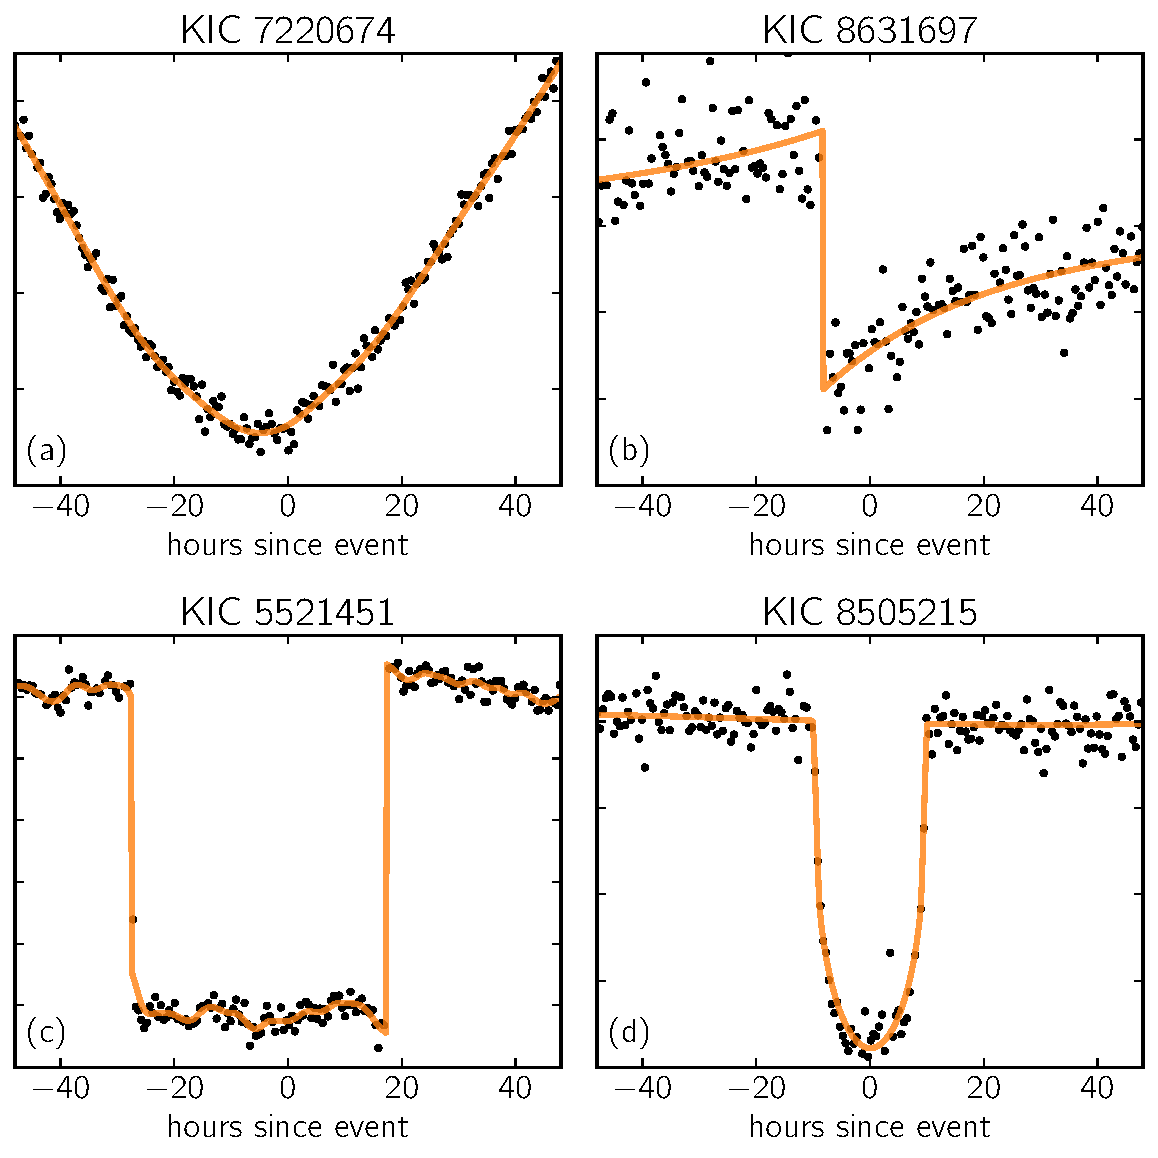
\includegraphics[width=\textwidth]{figures/model_comp.pdf}
\end{center}
\caption{%
Representative examples of candidate events flagged by the initial search.
Each example falls into a different model category and the figure shows the
data as black points and the best fit mean model prediction.
The examples represent the following model categories:
\emph{(a)} variability, \emph{(b)} step, \emph{(c)} box, and \emph{(d)}
transit.
\dfmfiglabel{model-comp}}
\end{figure*}


\subsection{Step 3 -- Pixel-level vetting}

To minimize contamination from background eclipsing binary systems, we require
candidate events to pass a centroid shift test similar to the one used in the
official \kepler\ transit search pipeline \citep{Bryson:2013}.
To measure the centroid shift, we model the flux-weighted centroid traces
independently in each coordinate as a multiple of the best-fit transit model
and a GP noise model.
By properly normalizing the transit model, we  measure the in-transit centroid
shift $\Delta_\mathrm{centroid}$ in pixels.
We reject any candidate event where the estimated transit location is more
than half a pixel from the out-of-transit centroid
\begin{eqnarray}
\Delta_\mathrm{centroid}\,\left(\frac{1}{\delta} - 1\right) &>& 0.5
\end{eqnarray}
where $\delta$ is the observed transit depth \citep{Bryson:2013}.


\section{Results: a catalog of long-period transiting exoplanet candidates}

To limit the scope of this paper while still demonstrating the applicability
of our method, we search the \kepler\ archival light curves of the brightest
and quietest Sun-like stars for long-period transiting exoplanets.
In this section, we describe the target selection process, the parameter
estimation procedure, and present the catalog of discoveries.


\subsection{Target selection}\sectlabel{target-selection}

We select the $\sim40,000$ brightest and quietest G and K dwarfs from the
\kepler\ catalog using the most recent catalog of stellar parameters%
\footnote{Parameters from the \textsf{q1\_q17\_dr24\_stellar} table from the
NASA Exoplanet Archive \citep[][with updates]{Huber:2014}.} and the cuts used
by \citet{Burke:2015}:
\begin{itemize}
{\item $4200\unit{K} \le T_\mathrm{eff} \le 6100\unit{K}$,}
{\item $R_\star \le 1.15\,R_\odot$,}
{\item $\mathrm{data\,span} \ge 2\,\mathrm{years}$,}
{\item $\mathrm{duty\,cycle} \ge 0.6$,}
{\item $K_p \le 15\unit{mag}$, and}
{\item $\mathrm{CDPP}_{7.5\unit{hrs}} \le 1000\unit{ppm}$.}
\end{itemize}
We continue by excluding the light curves of known eclipsing
binaries\footnote{\url{http://keplerebs.villanova.edu/}} \citep{Kirk:2016},
other known false positives \citep{Coughlin:2016}, a planet with known transit
timing variations (Kepler-9), and four especially noisy stars (KIC~4482348,
KIC~4450472, KIC~5438845, and KIC~10068041).
The final catalog contains \numtargets\ targets and the parameter distribution
is shown in \dfmfig{targets}.

Since these data have already been searched for short-period planets, we
assume that all high signal-to-noise candidates with three or more transits
have been previously found \citep{Coughlin:2016}.
To remove these candidates from consideration, we mask the cadences within two
transit durations of the time when a short-period planet candidate is known to
transit\footnote{We specifically use the \textsf{q1\_q17\_dr24\_koi} from the
NASA Exoplanet Archive \url{http://exoplanetarchive.ipac.caltech.edu/}.}.

\begin{figure}~\\
\begin{center}
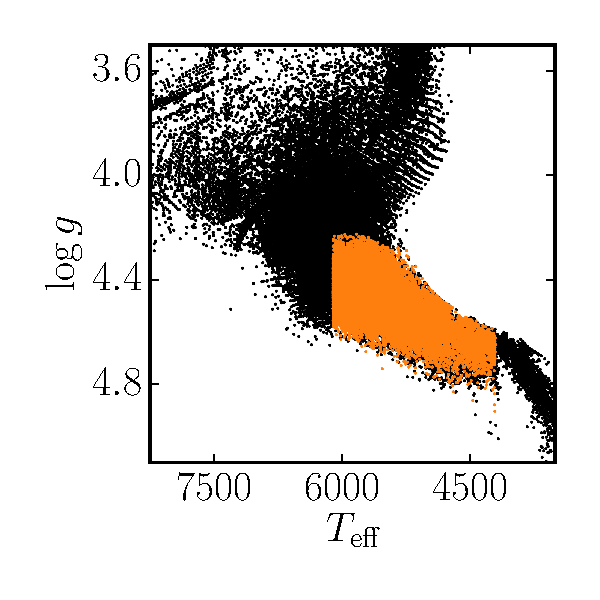
\includegraphics{figures/targets.pdf}
\end{center}
\caption{%
The distribution of stellar parameters for \kepler\ targets selected for this
search (orange) compared to the distribution of the full \kepler\ target
catalog (black).
\dfmfiglabel{targets}}~\\
\end{figure}


\subsection{Parameter estimation}

For each transit candidate, we constrain the physical parameters of the system
by fitting a section of light curve around each transit using an exposure time
integrated  Keplerian orbit with a quadratic limb darkening law for the
central body\footnote{Implemented at \url{https://github.com/dfm/transit};
this \paper\ uses git commit \textsf{482d99b} of that repository.}.
It has previously been established that the orbital period of a transiting
planet with only one transit can still be constrained given a measurement of
the stellar density and an assumption about the orbital eccentricity \cite[for
example][]{Wang:2015, Osborn:2016}.
Qualitatively this works because the transit of a bound body cannot have an
arbitrary period for a given duration.
This is the same argument used to justify the ``photoeccentric effect''
\citep{Dawson:2012} and the method of ``asterodensity profiling''
\citep{Kipping:2014b}.
In particular, this suggests that the periods of single transits in systems
with multiple inner planets will be especially well constrained
\citep{Kipping:2012}.
In this \paper, we do not take advantage of the extra constraints provided by
the inner planets, instead treating each long-period transiting system in
isolation, but this would be a good follow-up project.

In the following paragraphs, we describe the components of the probabilistic
model.
To perform parameter estimation under this model, we use the Markov Chain
Monte Carlo (MCMC) package \emcee\footnote{\url{http://dfm.io/emcee}}
\citep{Foreman-Mackey:2013} with an ensemble of 40 walkers.
We run each chain until at least 750 independent samples~--~in most cases, we
actually produce thousands of independent samples~--~are obtained\footnote{The
integrated autocorrelation time is estimated using a robust iterative method
as suggested by Alan Sokal:
\url{http://www.stat.unc.edu/faculty/cji/Sokal.pdf}.} and discard the first
third of the chain as burn-in.


\paragraph{Priors}

For each candidate in our sample, we take the constraints on the stellar
parameters from the \kepler\ stellar properties catalog\footnote{The
\textsf{q1\_q17\_dr24\_stellar} table from the NASA Exoplanet Archive
\citep{Huber:2014}} and assume an empirical beta function prior on the
eccentricities based on the observed eccentricity distribution of long-period
planets discovered using radial velocities \citep{Kipping:2013}.
Table~\ref{tab:parameters} lists all the fit parameters and their prior
distributions.
Besides these listed priors, we add the extra constraint that no other
transits can occur in the baseline of the \kepler\ observations.
This constraint is overly conservative because there is some probability that
a second transit could occur in a data gap but we find that, in practice, most
of the posterior mass is at longer periods and the period inferences are not
significantly affected.

\paragraph{Likelihood function}

As above, we model the light curve as GP with a physical transit model as the
mean and a covariance matrix described by a Mat\'ern-3/2 kernel function.
The full likelihood function and some details of GP regression are given in
\app{gp-regression}.
For computational efficiency, we first perform a joint optimization of the
physical parameters and GP hyperparameters to find the maximum \foreign{a
posteriori} model then keep the hyperparameters fixed and run MCMC sampling
for the 11 physical parameters alone.


\begin{floattable}
\begin{deluxetable}{lccc}
\tabletypesize{\footnotesize}
\caption{The inferred parameters and priors used in the inference
\label{tab:parameters}}

\tablehead{%
    \colhead{name} & \colhead{symbol} & \colhead{units} &
    \colhead{prior}
}

\startdata
mean flux & $\log f_\star$ & \nodata &
    $\log f_\star \sim \mathcal{U}(-1,\,1)$ \\
stellar mass\tablenotemark{a} & $M_\star$ & $M_\odot$ &
    $M_\star \sim \mathcal{N}(M_{\star,\mathrm{cat}},\,
        \sigma_{M,\star,\mathrm{cat}})$ \\
stellar radius\tablenotemark{a} & $R_\star$ & $R_\odot$ &
    $R_\star \sim \mathcal{N}(R_{\star,\mathrm{cat}},\,
        \sigma_{R,\star,\mathrm{cat}})$ \\
\multirow{2}{*}{limb darkening} & $q_1$ & \nodata &
    $q_1 \sim \mathcal{U}(0,\,1)$ \\
 & $q_2$ & \nodata & $q_2 \sim \mathcal{U}(0,\,1)$ \\
\hline
planet radius & $\log R_\mathrm{P}$ & $R_\odot$ &
    $\log R_\mathrm{P} \sim \mathcal{U}(-10,\,2)$ \\
reference time & $t_0$ & days &
    $t_0 \sim \mathcal{U}(t_\mathrm{cand}-0.5,\,t_\mathrm{cand}+0.5)$%
    \tablenotemark{b} \\
\multirow{2}{*}{\begin{minipage}{1in}semi-major axis \ \& inclination\end{minipage}}
    & $\sqrt{a}\sin i$ & ${R_\odot}^{1/2}$ &
    $\sqrt{a}\sin i \sim \mathcal{U}(-10^3,\,10^3) / \sqrt{a}$ \\
    & $\sqrt{a}\cos i$ & ${R_\odot}^{1/2}$ &
    $\sqrt{a}\cos i \sim \mathcal{U}(0,\,10^3) / \sqrt{a}$ \\
\multirow{2}{*}{eccentricity}
    & $\sqrt{e}\sin \omega$ & \nodata & $e \sim \beta(1.12,\,3.09)$%
    \tablenotemark{c} \\
    & $\sqrt{e}\cos \omega$ & \nodata & $\omega \sim \mathcal{U}(-\pi,\,\pi)$\\
\enddata

\tablenotetext{a}{Stellar parameters and uncertainties taken from the \kepler\
catalog \citep{Huber:2014}}
\tablenotetext{b}{The reference time is constrained to be within half a day of
the candidate transit time}
\tablenotetext{c}{\citet{Kipping:2013a}}
\tablecomments{There is one further constraint that complicates these priors:
the period of the orbit must be longer than some minimum period
$P_\mathrm{min}$ set by the transit time and the full baseline of \kepler\
observations.}
\end{deluxetable}
\end{floattable}



\subsection{Catalog of transit candidates}\sectlabel{catalog}

Applying the search procedure described in \sect{search} to the \kepler\ light
curves of the \numtargets\ targets selected in \sect{target-selection}, we
find \numcands\ convincing transit candidates.
Visual inspection of each candidate confirms the reliability of the
classification and no candidates are manually removed from the catalog.
Of these, three candidates have two transits in the \kepler\ baseline and the
remainder have only one observable transit.
The candidates and their inferred physical parameters are listed in
Table~\ref{tab:catalog} and the light curves are plotted in
\dfmfig{light-curves}.
The inferred radius and orbital periods of the candidates are compared to the
short-period \kepler\ sample and the Solar System in \dfmfig{full-sample}.

Two of the shortest period candidates~--~both with two observed
transits~--~have previously been studied in detail \citep[KIC~8800954 and
KIC~3239945;][]{Kipping:2014a, Kipping:2016}.
Table~\ref{tab:catalog} indicates the candidates that were also discovered by
earlier searches for long-period transiting systems using visual inspection
\citep{Wang:2015, Uehara:2016}.
The consistency between our results and the earlier catalogs is reassuring.
Our automated search did not find any more candidates than visual inspection
of the light curves of known KOIs \citep{Uehara:2016} and one candidate
(KIC~3230491) reported by the human analysis was discarded as grazing by our
search.
The PH citizen science project reported five long-period candidates with one
or two observed transits in our target list \citep{Wang:2015}.
Of these, we also find two (KIC~8410697 and KIC~10842718) although we find a
second transit in the KIC~8410697 system that was not previously reported.
The three other candidates reported by \citet{Wang:2015} that we miss
(KIC~5536555, KIC~9662267, and KIC~12454613) are have low signal-to-noise
transits that do not pass our initial signal-to-noise threshold.
Six of the candidates in Table~\ref{tab:catalog} have not been previously
published.

The candidate in the light curve of KIC~4754460 as an individual transit
candidate but another deeper eclipse can be found at a KBJD of 1587.13; right
at the beginning of Quarter 17.
This eclipse was missed by the automated search because only the second half
of the eclipse is observed.
The most likely explanation of this system is that the listed candidate is the
secondary eclipse of a binary system but we will keep the candidate is the
list and treat this effect statistically in \sect{false-positives}.

\begin{floattable}
\begin{deluxetable}{ccccccccl}
\tabletypesize{\footnotesize}
\caption{The inferred parameters for the long-period transiting exoplanet
candidates \label{tab:catalog}}
\tablehead{
    \colhead{kic id} & \colhead{period [years]} & \colhead{$t_0$ [KBJD]} &
    \colhead{radius [$R_\mathrm{J}$]} & \colhead{$T_\mathrm{eq}$ [K]} &
    \colhead{comments}
}
\startdata
3218908 & $7.0_{-3.4}^{+9.5}$ & $766.6722_{-0.0114}^{+0.0096}$ & $0.514_{-0.093}^{+0.092}$ & $129_{-39}^{+41}$ & KOI 1108 / Kepler-770\\
3239945 & $2.9328721(26)$ & $420.28714_{-0.00068}^{+0.00069}$ & $0.876\pm0.039$ & $142.8_{-4.2}^{+4.3}$ & KOI 490 / Kepler-167\\
4754460 & $5.9_{-3.0}^{+11.8}$ & $826.8369\pm0.0046$ & $0.67_{-0.15}^{+0.16}$ & $171_{-64}^{+59}$ & \\
6551440 & $4.0_{-1.2}^{+4.2}$ & $1039.0589\pm0.0037$ & $0.282_{-0.083}^{+0.093}$ & $170_{-45}^{+38}$ & \\
8410697 & $2.8688097(54)$ & $542.1231\pm0.0013$ & $0.698_{-0.078}^{+0.107}$ & $206_{-13}^{+15}$ & \\
8426957 & $54_{-36}^{+88}$ & $784.677\pm0.013$ & $1.04_{-0.25}^{+0.30}$ & $85_{-28}^{+46}$ & \\
8505215 & $9.1_{-3.4}^{+9.5}$ & $140.0492_{-0.0018}^{+0.0017}$ & $0.277\pm0.017$ & $103_{-23}^{+19}$ & \\
8738735 & $9.9_{-5.0}^{+14.9}$ & $697.8538_{-0.0049}^{+0.0059}$ & $0.355_{-0.044}^{+0.045}$ & $136_{-39}^{+43}$ & KOI 693 / Kepler-214\\
8800954 & $1.9279957(91)$ & $492.7652\pm0.0024$ & $0.386\pm0.025$ & $189.4_{-7.3}^{+7.2}$ & KOI 1274 / Kepler-421\\
9306307 & $4.2_{-1.1}^{+3.2}$ & $1191.35648\pm0.00018$ & $1.20_{-0.33}^{+0.51}$ & $127\pm32$ & \\
10187159 & $4.9_{-1.8}^{+7.6}$ & $604.1102_{-0.0031}^{+0.0023}$ & $0.43_{-0.13}^{+0.21}$ & $119_{-43}^{+34}$ & KOI 1870 / Kepler-989\\
10287723 & $4.9_{-1.3}^{+4.3}$ & $393.5976_{-0.0029}^{+0.0031}$ & $0.266_{-0.024}^{+0.027}$ & $114_{-21}^{+13}$ & \\
10321319 & $5.5_{-2.1}^{+8.1}$ & $554.3562_{-0.0063}^{+0.0064}$ & $0.163_{-0.037}^{+0.046}$ & $153_{-47}^{+37}$ & \\
10602068 & $3.15_{-0.82}^{+2.79}$ & $830.80892\pm0.00015$ & $1.99_{-0.34}^{+0.66}$ & $158_{-34}^{+30}$ & \\
10842718 & $12.7_{-6.6}^{+20.2}$ & $226.2344\pm0.0047$ & $0.74\pm0.16$ & $128_{-43}^{+47}$ & \\
11709124 & $4.3_{-1.3}^{+4.7}$ & $657.2674_{-0.0016}^{+0.0018}$ & $0.83_{-0.11}^{+0.12}$ & $166_{-39}^{+28}$ & KOI 435 / Kepler-154\\
\enddata

\tablenotetext{*}{The equilibrium temperature is computed assuming zero
albedo.}
\tablenotetext{\dagger}{Candidate has two observed transits.}
\tablenotetext{a}{Included in the \citet{Wang:2015} catalog.}
\tablenotetext{b}{Included in the \citet{Uehara:2016} catalog.}
\tablecomments{The values and uncertainties indicate the 16-th, 50-th, and
84-th percentiles of the posterior samples for each parameter.}
\end{deluxetable}
\end{floattable}

\begin{figure*}[p]~\\
\begin{center}
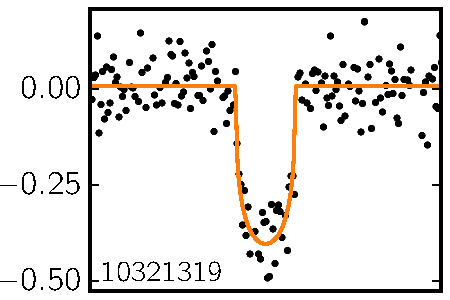
\includegraphics[width=0.24\textwidth]{figures/lcs/10321319.pdf}
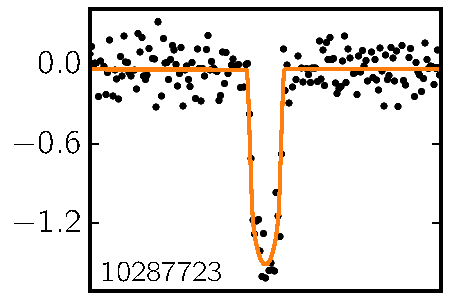
\includegraphics[width=0.24\textwidth]{figures/lcs/10287723.pdf}
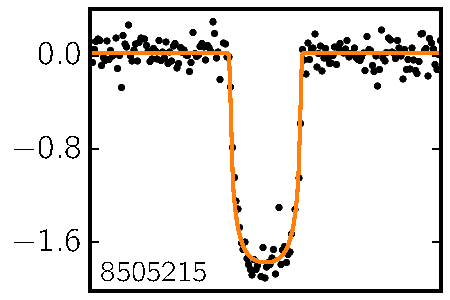
\includegraphics[width=0.24\textwidth]{figures/lcs/8505215.pdf}
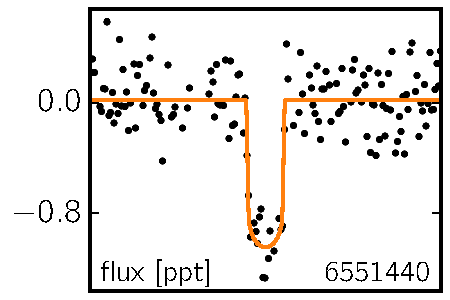
\includegraphics[width=0.24\textwidth]{figures/lcs/6551440.pdf}
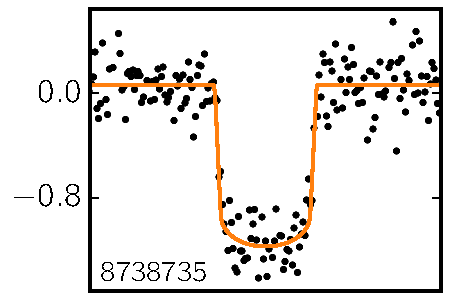
\includegraphics[width=0.24\textwidth]{figures/lcs/8738735.pdf}
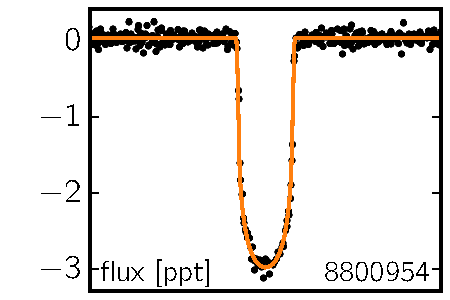
\includegraphics[width=0.24\textwidth]{figures/lcs/8800954.pdf}
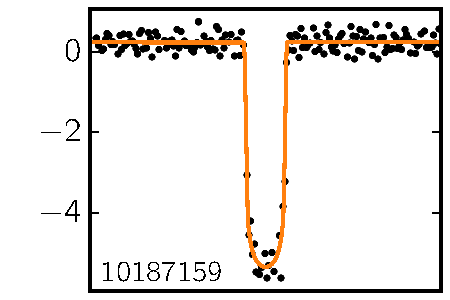
\includegraphics[width=0.24\textwidth]{figures/lcs/10187159.pdf}
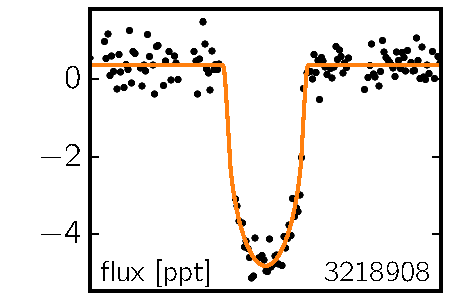
\includegraphics[width=0.24\textwidth]{figures/lcs/3218908.pdf}
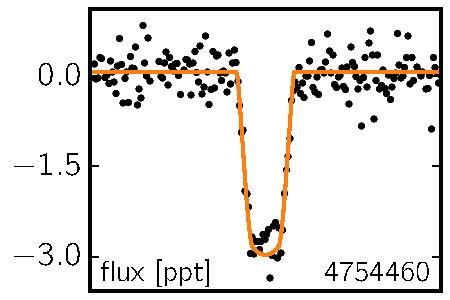
\includegraphics[width=0.24\textwidth]{figures/lcs/4754460.pdf}
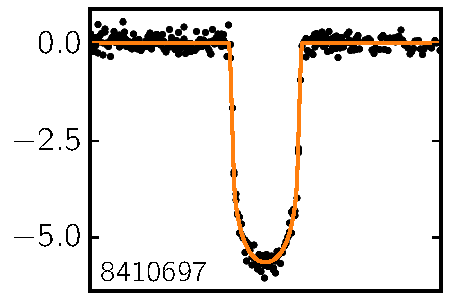
\includegraphics[width=0.24\textwidth]{figures/lcs/8410697.pdf}
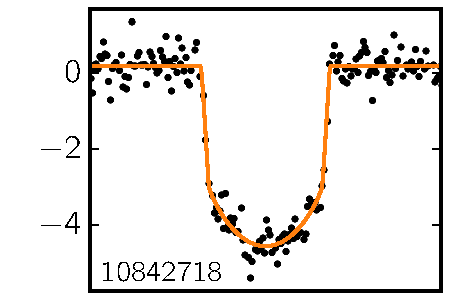
\includegraphics[width=0.24\textwidth]{figures/lcs/10842718.pdf}
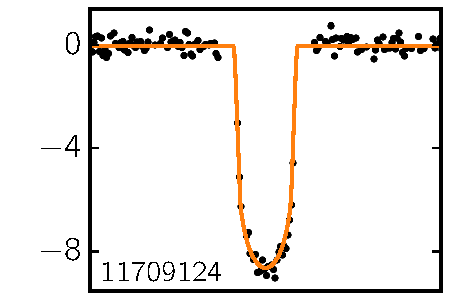
\includegraphics[width=0.24\textwidth]{figures/lcs/11709124.pdf}
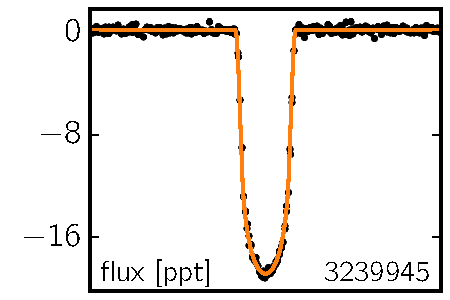
\includegraphics[width=0.24\textwidth]{figures/lcs/3239945.pdf}
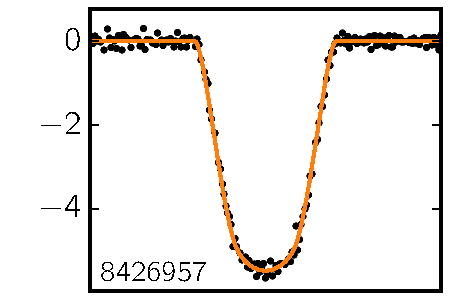
\includegraphics[width=0.24\textwidth]{figures/lcs/8426957.pdf}
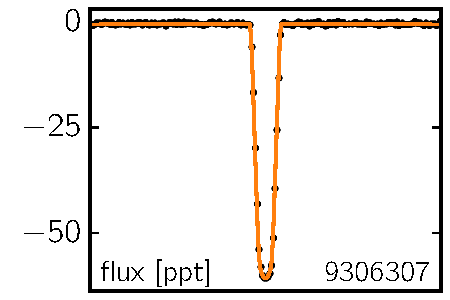
\includegraphics[width=0.24\textwidth]{figures/lcs/9306307.pdf}
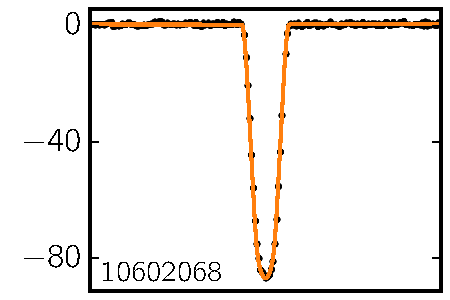
\includegraphics[width=0.24\textwidth]{figures/lcs/10602068.pdf}

\end{center}
\caption{%
Sections of \pdc\ light curve centered on each candidate (black) with the
posterior-median transit model over-plotted (orange).
Candidates with two transits are folded on the posterior-median period.
The plots are ordered by increasing planetary radius from the top-left to the
bottom-right.
\dfmfiglabel{light-curves}}
\end{figure*}

\begin{figure*}~\\
\begin{center}
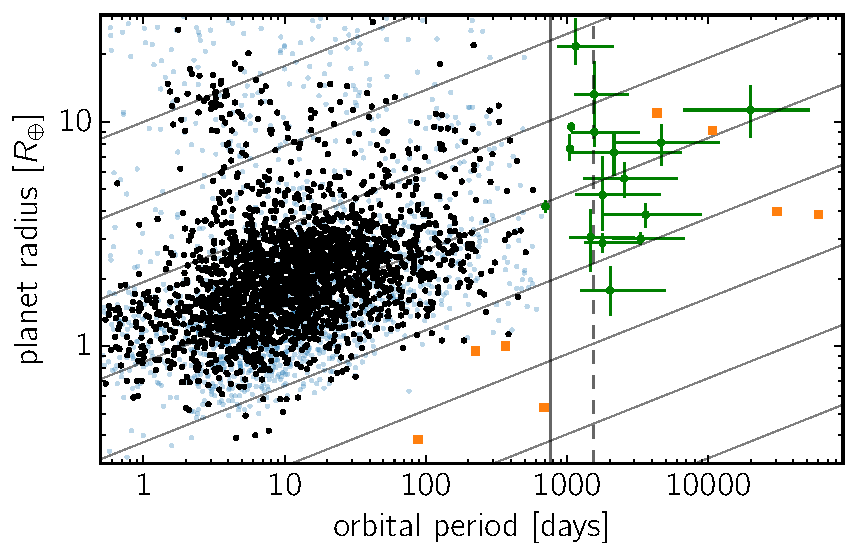
\includegraphics{figures/full_sample_plus_cands.pdf}
\end{center}
\caption{%
The catalog of long-period transiting exoplanet candidates (green) compared to
the \kepler\ candidates (blue) and confirmed planets (black), and the Solar
System (orange).
The vertical dashed line indicates the full lifetime of the \kepler\ Mission;
planets with orbital periods longer than this will show at most one transit.
The vertical solid line shows the absolute maximum period accessible to
transit searches that require at least three transits.
\dfmfiglabel{full-sample}}~\\
\end{figure*}



\section{Empirical search completeness}\sectlabel{completeness}

To measure the completeness of search procedure described in \sect{search}, we
exploit the fact that transit signals are sparse and rare.
Therefore, most light curves contain no transits and we can reliably measure
the recovery rate of our method on synthetic transit signals~--~with known
properties~--~injected into real light curves.
This procedure is standard practice in the transit literature and it has been
used to determine the completeness of the KOI catalog
\citep{Christiansen:2013, Christiansen:2015} and other independent transit
searches \citep{Petigura:2013, Dressing:2015, Foreman-Mackey:2015}.

To reliably capture the full structure of the search completeness function,
the simulations must sample the (high-dimensional) space of all properties
that affect the probability of detecting a transit: the stellar properties
(including variability amplitudes and time scales), the planet's physical
properties and orbital elements, and any observational effects (noise,
spacecraft pointing variations, \etc).
For the modest goals of this paper, we only need a robust constraint on the
transit detection efficiency \emph{integrated} across the target sample but,
even so, many simulations per star are required.

The procedure for measuring the recovery rate of simulated transits is as
follows:
\begin{enumerate}
{\item First, a star is randomly selected from the target list, and the \pdc\
light curve and stellar properties for that star are loaded.}
{\item Planetary properties are sampled from the distributions listed in
Table~\ref{tab:simulations} with phase uniformly distributed across the
baseline of observations. These properties are re-sampled until the transit is
visible in at least one non-flagged cadence.}
{\item The transit signal induced by this planet is computed and multiplied
into the \pdc\ light curve.}
{\item The transit search method described in \sect{search}~--~including
de-trending and all automated vetting~--~is applied to this light
curve with the injected transit signal.}
{\item This candidate is flagged as recovered if at least one transit within
one transit duration passes all the cuts imposed by the automated vetting.}
\end{enumerate}

The fraction of recovered simulations as a function of the relevant parameters
gives an estimate of the search completeness or the probability of detecting
an exoplanet transit with a given set of parameters, \emph{conditioned on the
fact that it transits}.
We will call this function $Q_{\mathrm{det},k}(\params)$ where \params\ is the
set of all parameters affecting the transit detectability and $k$ is an index
running over target stars.

\dfmfig{completeness} shows the fraction of recovered simulations as a
function of planet radius and orbital period based on \numinjs\ injected
signals.
This figure shows the transit detection efficiency falling with decreasing
planet radius.
This is the expected behavior because the depth (and signal strength) of a
transit scales with the area ratio between the planet and the star.
The decreasing completeness with orbital period is less intuitive because, on
average, the signal strength should increase as the duration of the transit
increases.
In this case, this simplistic treatment misses two important factors.
First, in step 1 of the search procedure (\sect{stepone}) only a single
transit duration is used and second, longer transits are less easily
distinguished from stellar variability and they will, therefore, be discarded
in the conservative light curve vetting step (\sect{light-curve-vetting}).

This detection efficiency must then be combined with the geometric transit
probability function and the window function.
For the star $k$, the geometric transit probability is given by
\citep{Winn:2010}
\begin{eqnarray}
Q_{\mathrm{geom},k} (\params) &=& \frac{R_{\star,k} + R}{a_k}
    \, \frac{1 + e\,\sin\omega}{1-e^2} \\
&=& \left[\frac{4\,\pi^2}{G\,M_{\star,k}}\right]^{1/3}\,(R_{\star,k}+R)
    \, \left[\frac{1 + e\,\sin \omega}{1-e^2}\right]
    \, P^{-2/3}
\end{eqnarray}
where $R$ is the planet radius, $P$ is the orbital period, $e$ is the orbital
eccentricity, $\omega$ is the argument of periastron, $R_{\star,k}$ is
the radius of star $k$, and $M_{\star,k}$ is the star's mass.
All of these parameters are included in \params.

Approximating the window function using a binomial probability of observing
at least one transit, we find \citep[following][]{Burke:2014a}
\begin{eqnarray}
Q_{\mathrm{win},k} (\params) &=& 1 - (1 - f_{\mathrm{duty},k})^{T_k/P}
\end{eqnarray}
where $f_{\mathrm{duty},k}$ is the duty cycle and $T_k$ is the full
observation baseline for target $k$.

Combining these detection effects, the total detection efficiency is given by
\begin{eqnarray}
Q_k(\params) &=& Q_{\mathrm{det},k}(\params) \,
                 Q_{\mathrm{win},k} (\params) \,
                 Q_{\mathrm{geom},k} (\params) \quad.
\end{eqnarray}

So that our planet candidate catalog can be easily used for other projects, we
also provide an analytic approximation to the relevant integrated detection
efficiency function
\begin{eqnarray}
Q_\mathrm{det}(P,\,R) &=& \sum_{k=1}^{K} \int Q_\mathrm{det,k}(\params)\,
    p(\params_{\{P,\,R\}}) \dd\params_{\{P,\,R\}}
\end{eqnarray}
where $p(\params_{\{P,\,R\}})$ is the prior distribution of all the parameters
except the period and radius.
We find that a good fit to this integrated completeness is given by the
function
\begin{eqnarray}
Q_\mathrm{det}(P,\,R) &\approx&
    \frac{\mathrm{min}[\mathrm{max}[a(P)\,b(R),\,0],\,1]}
         {1+\exp\left[-k(P)\,(\ln R-x(P))\right]}
\end{eqnarray}
where
\begin{eqnarray}
a(P) = a_1\,\ln P + a_2 \,,\quad
b(R) = b_1\,\ln R + b_2 \,,\quad \\
k(P) = k_1\,\ln P + k_2 \,,\,\mathrm{and}\quad
x(P) = x_1\,\ln P + x_2 \,.
\end{eqnarray}
When fit to the set of \numinjs\ injected transits, the best fit parameters
are given in Table~\ref{tab:completeness} and the approximation is plotted
in \dfmfig{completeness-analytic}.
Note that we do not use this approximation in the following analysis but
instead compute the relevant integrals using the injection catalog directly.


\begin{floattable}
\begin{deluxetable}{lc}
\tabletypesize{\footnotesize}
\caption{Distributions of physical parameters for transit simulations
\label{tab:simulations}}

\tablehead{%
    \colhead{name} & \colhead{distribution}
}
\startdata
period & $\log P \sim \mathcal{U}(\log 2\unit{yr},\,\log 25\unit{yr})$ \\
radius ratio & $\log R_\mathrm{P}/R_\star \sim
    \mathcal{U}(\log 0.02,\,\log 0.2)$ \\
impact parameter & $b \sim \mathcal{U}(0,\,1+R_\mathrm{P}/R_\star)$ \\
\multirow{2}{*}{eccentricity} & $e \sim \beta(1.12,\,3.09)$\tablenotemark{a} \\
    & $\omega \sim \mathcal{U}(-\pi,\,\pi)$\\
\multirow{2}{*}{limb darkening} & $q_1 \sim \mathcal{U}(0,\,1)$ \\
                                & $q_2 \sim \mathcal{U}(0,\,1)$ \\
\enddata

\tablenotetext{a}{\citet{Kipping:2013a}}
\end{deluxetable}
\end{floattable}

\begin{figure*}[p]~\\
\begin{center}
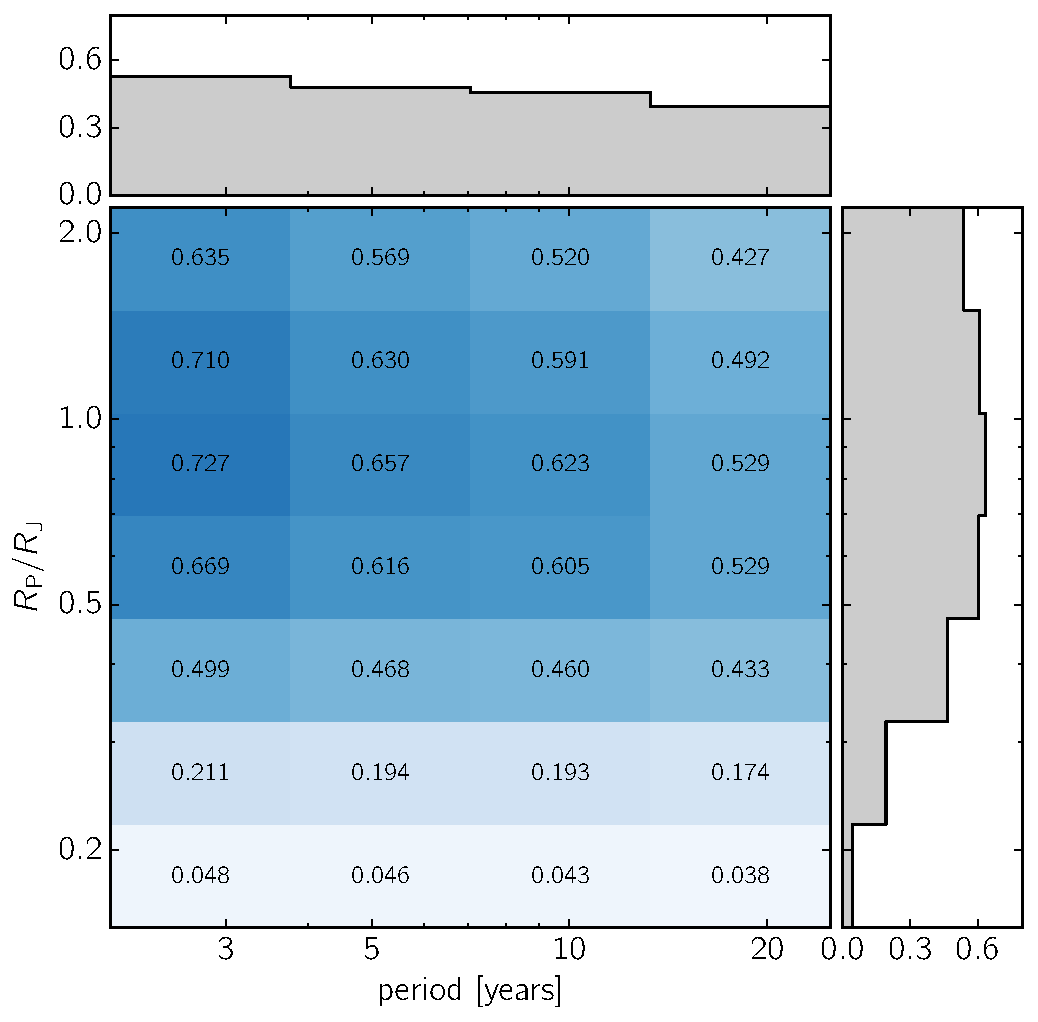
\includegraphics[width=\textwidth]{figures/completeness.pdf}
\end{center}
\caption{%
An empirical estimate of the search completeness as a function of planet
radius and orbital period.
In each bin, the completeness is estimated by the fraction of recovered
simulations.
The projected histograms show the integrated completeness as independent
functions of period and radius.
\dfmfiglabel{completeness}}
\end{figure*}

\begin{figure*}[htbp]~\\
\begin{center}
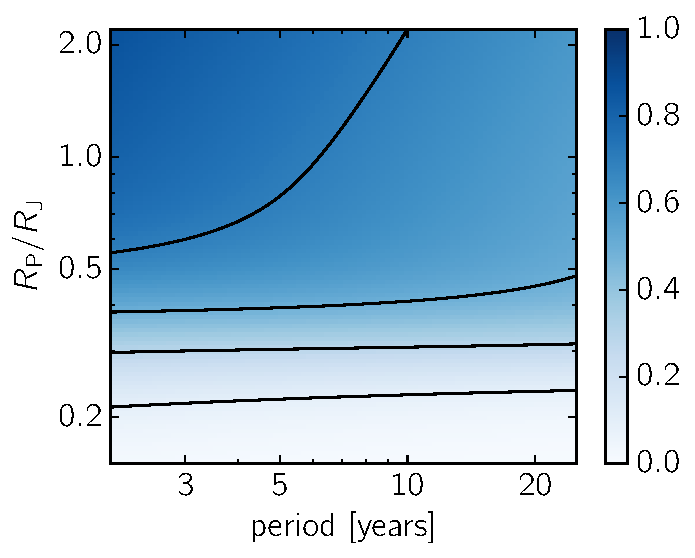
\includegraphics[width=0.6\textwidth]{figures/completeness_analytic.pdf}
\end{center}
\caption{%
An analytic approximation to \dfmfig{completeness} with the same color scale.
The contours indicate the 0.1, 0.3, 0.5, and 0.7 levels.
\dfmfiglabel{completeness-analytic}}
\end{figure*}

\begin{floattable}
\begin{deluxetable}{cc|cc}
\tabletypesize{\footnotesize}
\caption{The fit parameters for the analytic approximation to the completeness
function
\label{tab:completeness}}
\tablehead{%
    \colhead{parameter} & \colhead{value} &
    \colhead{parameter} & \colhead{value}
}
\startdata
$a_1$ & $\paramc$ & $k_1$ & $\parame$ \\
$a_2$ & $\paramd$ & $k_2$ & $\paramf$ \\
$b_1$ & $\parama$ & $x_1$ & $\paramg$ \\
$b_2$ & $\paramb$ & $x_2$ & $\paramh$ \\
\enddata
\end{deluxetable}
\end{floattable}


\section{The occurrence rate of long-period exoplanets}

Using the catalog of exoplanet discoveries (\sect{catalog}) and the
measurement of the search completeness (\sect{completeness}), we can now
estimate the occurrence rate of long-period exoplanets.
To simplify the analysis, we will make the strong assumption that none of the
candidates are astrophysical false positives (the eclipse of a stellar mass
companion, a background eclipsing binary, or the secondary eclipse of a
long-period binary system).
We revisit this assumption and discuss its validity in the following section.
As a further simplification, we also neglect the measurement uncertainties on
the planet parameters (including orbital period).
This assumption is only justified because we are only making high-level
measurements of the mean occurrence rate in large bins.

Assuming a Poisson likelihood, the occurrence rate density in a volume
$V$~--~defined as $P_\mathrm{min} \le P < P_\mathrm{max}$ and
$R_\mathrm{min} \le R < R_\mathrm{max}$~--~is
\citep[see, for example, the Appendix of][]{Foreman-Mackey:2014}
\begin{eqnarray}\eqlabel{rate-density}
\Gamma_V \equiv \frac{\dd N}{\dd\ln P\dd\ln R} &=&
    \frac{C(P_\mathrm{min},\,P_\mathrm{max};\,R_\mathrm{min},\,R_\mathrm{max})}
         {Z(P_\mathrm{min},\,P_\mathrm{max};\,R_\mathrm{min},\,R_\mathrm{max})}
\end{eqnarray}
where $N$ is the expected number of planets per G/K dwarf, $C(\cdots)$ is the
number of detected planets in the volume, and
\begin{eqnarray}
Z(P_\mathrm{min},\,P_\mathrm{max};\,R_\mathrm{min},\,R_\mathrm{max}) &=&
    \sum_{k=1}^{K} \int p(\params_{\{P,\,R\}})\,
    Q_k(\params)\,\bvec{1}[P,\,R\in V]\dd \params
\end{eqnarray}
where $p(\params_{\{P,\,R\}})$ is the prior distribution of all the parameters
except the period and radius and $\bvec{1}[\cdot]$ is 1 if the argument is
satisfied and 0 otherwise.
Using the $J$ injections sampled uniformly in period and radius and other
parameters from $p(w_{\{P,\,R\}})$,
\begin{eqnarray}
Z(P_\mathrm{min},\,P_\mathrm{max};\,R_\mathrm{min},\,R_\mathrm{max}) &\approx&
    \frac{K}{J}\,\sum_{j=1}^{J} Q_k(w^{(j)})
\end{eqnarray}
where the sum is over all injections in the volume $V$.

Using the injection results from \sect{completeness} and the catalog of
discoveries from \sect{catalog}, we compute the occurrence rate in the period
range 2 to 25 years and in two radius bins between 0.1 and
$1.0\,R_\mathrm{J}$.
The calculated occurrence rates are listed in Table~\ref{tab:occurrence}.

For comparison, we repeated the analysis of \citet{Burke:2015} and fit a
double power-law occurrence rate to the short-period \kepler\ planet
candidates\footnote{The analysis was adapted from publicly available code that
was demonstrated to reproduce the same results as \citet{Burke:2015} by
\citet{Foreman-Mackey:2015a}.} and extrapolated to the center of the two
bins where we computed the occurrence rate.
At a period of 7~years and a radius of $0.2\,R_\mathrm{J}$, the extrapolated
occurrence is $0.73\pm0.28$ and at a radius of $0.6\,R_\mathrm{J}$, the
extrapolated rate is $0.15\pm0.05$.

\begin{floattable}
\begin{deluxetable}{ccc}
\tabletypesize{\footnotesize}
\caption{The occurrence rate density in two radius bins \label{tab:occurrence}}
\tablehead{
    \colhead{$R_\mathrm{min}\,[R_\mathrm{J}]$} &
    \colhead{$R_\mathrm{max}\,[R_\mathrm{J}]$} &
    \colhead{$\Gamma_{R\in[R_\mathrm{min},\,R_\mathrm{max}],\,
              P\in[2\,\mathrm{yr},\,25\,\mathrm{yr}]}$\tablenotemark{a}}
}
\startdata
$0.1$ & $0.4$ & $0.24\pm0.11$ \\
$0.4$ & $1.0$ & $0.18\pm0.07$ \\
\enddata

\tablenotetext{a}{See \eq{rate-density}}
\tablecomments{These values are computed in the period range 2--25~years.}
\end{deluxetable}
\end{floattable}


\section{Astrophysical false positives}\sectlabel{false-positives}

Various configurations of grazing or blended eclipsing binaries can mimic the
signal of a transiting planet \citep{}. The occurrence rate calculation
presented in the preceding section assumes that none of the planet
candidates identified in this work are caused by such astrophysical false
positives.  In this Section we explore the validity of this assumption.


\section{Comparison with the literature}\sectlabel{comparison}


\begin{floattable}
\begin{deluxetable}{cccc}
\tabletypesize{\footnotesize}
\caption{The inferred parameters for the long-period transiting exoplanet
candidates \label{tab:masses}}
\tablehead{
    \colhead{kic id} &
    \colhead{radius} &
    \colhead{mass\tablenotemark{*}} &
    \colhead{semi-major axis} \\
    & \colhead{$R_\mathrm{J}$} & \colhead{$M_\mathrm{J}$} & \colhead{AU}
}
\startdata
3218908 & $0.514_{-0.093}^{+0.092}$ & $0.079_{-0.038}^{+0.074}$ & $3.4_{-1.2}^{+2.7}$\\
3239945 & $0.876_{-0.039}^{+0.039}$ & $6.5_{-6.3}^{+38.1}$ & $1.864_{-0.023}^{+0.025}$\\
4754460 & $0.67_{-0.15}^{+0.16}$ & $0.140_{-0.078}^{+9.248}$ & $3.1_{-1.2}^{+3.4}$\\
6551440 & $0.282_{-0.083}^{+0.093}$ & $0.028_{-0.015}^{+0.033}$ & $2.50_{-0.52}^{+1.55}$\\
8410697 & $0.698_{-0.078}^{+0.107}$ & $0.157_{-0.081}^{+11.710}$ & $1.925_{-0.038}^{+0.054}$\\
8426957 & $1.04_{-0.25}^{+0.30}$ & $3.8_{-3.7}^{+47.6}$ & $14.1_{-7.4}^{+13.0}$\\
8505215 & $0.277_{-0.017}^{+0.017}$ & $0.028_{-0.012}^{+0.022}$ & $4.0_{-1.1}^{+2.5}$\\
8738735 & $0.355_{-0.044}^{+0.045}$ & $0.042_{-0.019}^{+0.037}$ & $4.8_{-1.8}^{+4.0}$\\
8800954 & $0.386_{-0.025}^{+0.025}$ & $0.049_{-0.022}^{+0.039}$ & $1.420_{-0.028}^{+0.026}$\\
9306307 & $1.22_{-0.36}^{+0.49}$ & $4.5_{-4.2}^{+95.7}$ & $2.39_{-0.45}^{+1.09}$\\
10187159 & $0.43_{-0.13}^{+0.21}$ & $0.061_{-0.036}^{+0.096}$ & $2.70_{-0.69}^{+2.35}$\\
10287723 & $0.266_{-0.024}^{+0.027}$ & $0.026_{-0.012}^{+0.021}$ & $2.58_{-0.46}^{+1.35}$\\
10321319 & $0.163_{-0.037}^{+0.046}$ & $0.0120_{-0.0058}^{+0.0115}$ & $2.93_{-0.81}^{+2.44}$\\
10602068 & $2.00_{-0.35}^{+0.66}$ & $162_{-162}^{+74}$ & $2.11_{-0.40}^{+1.09}$\\
10842718 & $0.74_{-0.16}^{+0.16}$ & $0.19_{-0.12}^{+22.19}$ & $5.3_{-2.1}^{+4.7}$\\
11709124 & $0.83_{-0.11}^{+0.12}$ & $0.94_{-0.82}^{+35.47}$ & $2.54_{-0.56}^{+1.62}$\\
\enddata

\tablenotetext{*}{The equilibrium temperature is computed assuming zero
albedo.}
\end{deluxetable}
\end{floattable}

\begin{figure*}[p]~\\
\begin{center}
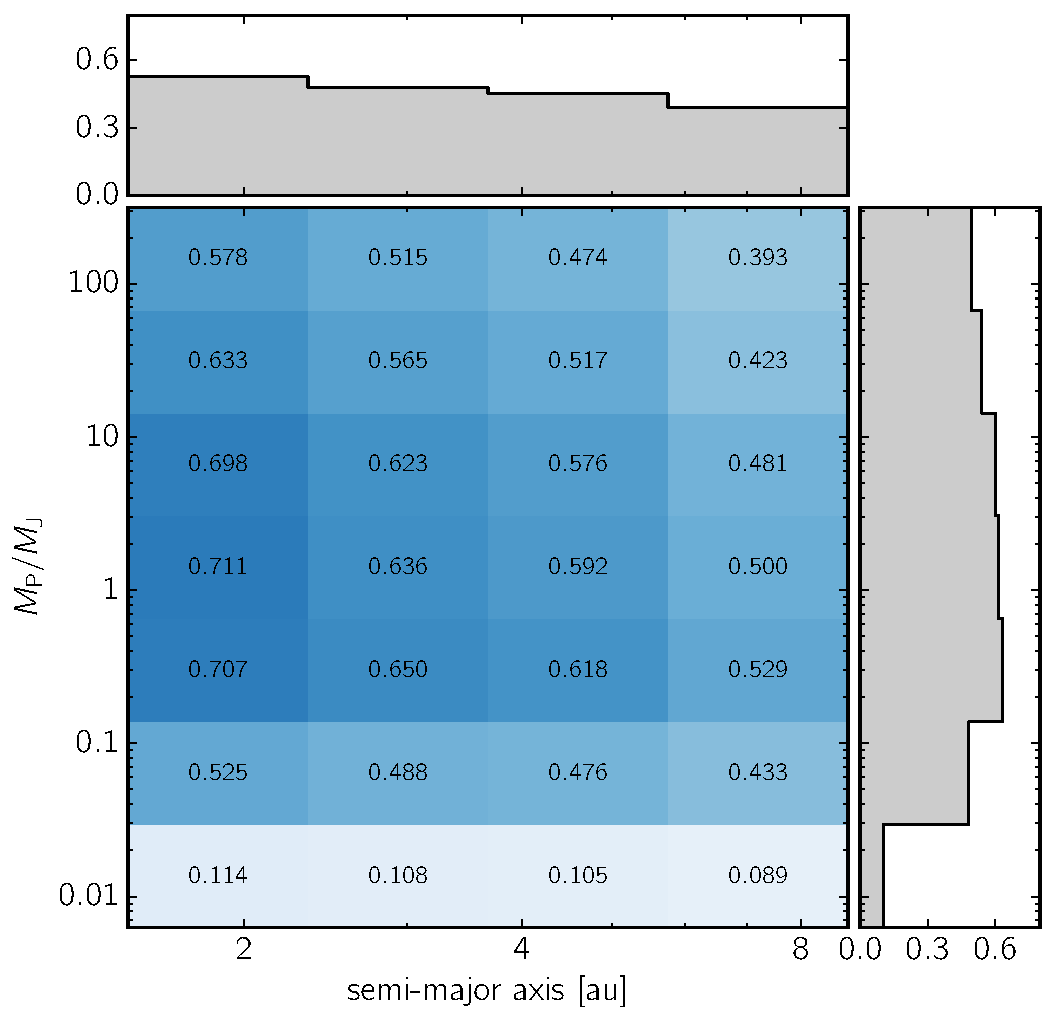
\includegraphics[width=\textwidth]{figures/completeness-am.pdf}
\end{center}
\caption{%
The same as \dfmfig{completeness} converted into the planet mass and
semi-major axis plane.
Since the completeness function depends on the planet's radius and not its
mass, a probabilistic mass--radius relation \citep{Chen:2016} was used to
convert radius to mass.
\dfmfiglabel{completeness-am}}
\end{figure*}


\section{Discussion}\sectlabel{discussion}

We have developed a fully automated method to search for the transits and
eclipses of long-period companions in photometric time series.
Applying this method to a subset of the \kepler\ archival light curves, we
discovered XX astrophysical transits.
Of these discoveries, at least about YY are likely to be planetary in nature.
Combining this catalog of discoveries with a measurement of the completeness
of our search method, we place a constraint on the occurrence rate of
long-period exoplanets.

Our method for transit detection finds convincing transit-shaped signals does
a model comparison between a physical transit model.

All of the code used in this project is available from
\url{https://github.com/dfm/peerless} under the MIT open-source software
license.
This code (plus some dependencies) can be run to re-generate all of the
figures and results in this \paper; this version of the paper was generated
with git commit \texttt{\githash} (\gitdate).


\acknowledgments
It is a pleasure to thank
\ldots
for helpful contributions to the ideas and code presented here.

DWH was partially supported by the National Science Foundation (grant
IIS-1124794), the National Aeronautics and Space Administration (grant
NNX12AI50G), and the Moore--Sloan Data Science Environment at NYU.

This research made use of the NASA \project{Astrophysics Data System} and the
NASA Exoplanet Archive.
The Exoplanet Archive is operated by the California Institute of Technology,
under contract with NASA under the Exoplanet Exploration Program.

This \paper\ includes data collected by the \kepler\ mission. Funding for the
\kepler\ mission is provided by the NASA Science Mission directorate.
We are grateful to the entire \kepler\ team, past and present.
Their tireless efforts were all essential to the tremendous success of the
mission and the successes of \KT, present and future.

These data were obtained from the Mikulski Archive for Space Telescopes
(MAST).
STScI is operated by the Association of Universities for Research in
Astronomy, Inc., under NASA contract NAS5-26555.
Support for MAST is provided by the NASA Office of Space Science via grant
NNX13AC07G and by other grants and contracts.

Computing resources were provided by High Performance Computing at New York
University.

\facility{Kepler}
\software{%
    \project{ceres} \citep{Agarwal:2016},
    \project{corner.py} \citep{Foreman-Mackey:2016},
    \project{emcee} \citep{Foreman-Mackey:2013},
    \project{george} \citep{Ambikasaran:2016},
	\project{matplotlib} \citep{Hunter:2007},
	\project{numpy} \citep{Van-Der-Walt:2011},
	\project{scipy} \citep{Jones:2001}}.

\newpage
\appendix

\section{Details of the light curve models}\sectlabel{model-details}

In \sect{light-curve-vetting}, the five light curve models were listed.
In this section, we give the mathematical details of each model and list the
parameters that are fit.
Each model~--~except the \modelname{transit} model~--~can be easily
differentiated with respect to its parameters.
As discussed in the following section, this feature is crucial for efficient
and robust likelihood maximization.

\begin{itemize}

{\item
The \modelname{box} model is given by
\begin{eqnarray}
m_\mathrm{box}(t) &=& \left\{\begin{array}{ll}
a, & \mbox{if $t \le t_\mathrm{min}$} \\
b, & \mbox{if $t_\mathrm{min} < t \le t_\mathrm{max}$} \\
c, & \mbox{if $t_\mathrm{max} < t$}
\end{array}\right.
\end{eqnarray}
where $a$, $b$, and $c$ are free parameters, and $t_\mathrm{min}$ and
$t_\mathrm{max}$ are fixed.
In practice, we include two different \modelname{box} models where
$t_\mathrm{min}$ and $t_\mathrm{max}$ are set using different heuristics.
The first \modelname{box} has the bounds set to match the ingress and
egress of the best fit \modelname{transit}.
The second \modelname{box} is chosen based on the largest change points in the
light curve.
}

{\item
The \modelname{step} model is given by
\begin{eqnarray}
m_\mathrm{step}(t) &=& \left\{\begin{array}{ll}
m_1 + h_1\,\exp\left([t - t_0] / w_1\right), & \mbox{if $t < t_0$} \\
m_2 + h_2\,\exp\left([t_0 - t] / w_2\right), & \mbox{if $t_0 \le t$}
\end{array}\right.
\end{eqnarray}
where all of the parameters~--~including $t_0$~--~are included in the fit.
To ensure that the widths $w_*$ remain positive, we fit for $\log w_*$.
}

{\item
For the \modelname{outlier} model, we iterate through all cadences $t_n$
within 0.3~days of the candidate transit time and evaluate the model as
\begin{eqnarray}
m_\mathrm{outlier}(t) &=& \left\{\begin{array}{ll}
f(t_0), & \mbox{if $t = t_0$} \\
\mathrm{median}[f(t \ne t_0)], & \mbox{if $t \ne t_0$}
\end{array}\right.
\end{eqnarray}
where $f(t)$ is the observed time series.
With this model, no non-linear optimization is required and the final value of
$t_0$ is the one with the maximum likelihood in this grid search.
}

{\item
The \modelname{variability} model only has one parameter, the flux $m_0$ and
$m_\mathrm{variability}(t) = m_0$ at all times.
The variability is captured by the Gaussian Process residual model.
}

{\item
Finally, the \modelname{transit} model is an exposure time integrated,
limb darkened light curve \citep{Mandel:2002, Kipping:2010} parameterized by
the radius ratio between the planet and star, the transit duration, the
transit time, the impact parameter, and two quadratic limb darkening
coefficients \citep{Kipping:2013}.
Analytically computing the gradient of a simple transit model is possible
\citep{Pal:2008} but it becomes substantially more tedious as the model
becomes more realistic.
Therefore, we instead use a compile-time automatic differentiation
library\footnote{More specifically, we use the \texttt{Jet} object from the
BSD-licensed Ceres Solver \url{http://ceres-solver.org}} \citep{Agarwal:2016}
to efficiently compute first derivatives of the full transit model with
respect to the orbital and physical parameters to machine precision.
}

\end{itemize}



\section{Gaussian process regression}\sectlabel{gp-regression}

Gaussian Processes (GPs) are a class of non-parametric, stochastic models that
have been demonstrated to be good effective models for the variability in
\kepler\ light curves.
A simple GP model can be used to capture residual non-transit variability in
light curves.
In this \paper, we use a GP model for two steps: light curve--level transit
shape vetting and parameter estimation.
A full discussion of GPs is beyond the scope of this \paper, so we will only
summarize the most relevant points here and direct an interested reader to
\citet{Rasmussen:2006} for more details.

A GP model is specified by the following likelihood function
\begin{eqnarray}\eqlabel{gplike}
\mathcal{L} = \ln p(\bvec{y}\,|\,\meanpars,\,\kernpars) &=&
- \frac{1}{2}\,\bvec{r}(\meanpars)^\T\,K(\kernpars)^{-1}\,
    \bvec{r}(\meanpars)
- \frac{1}{2}\log\det K(\kernpars) - \frac{N}{2} \log{2\,\pi}
\end{eqnarray}
where \bvec{y} is a list of measurements in a scalar time series~--~in this
case, fluxes~--~measured at the times \bvec{t}, and
\begin{eqnarray}
\bvec{r}(\meanpars) &=& \bvec{y} - m(\bvec{t};\,\meanpars)
\end{eqnarray}
is the vector of residuals away from the mean model $m(\bvec{t};\,\meanpars)$.
For the purposes of this paper, we model the covariance matrix $K(\kernpars)$
using the Mat\'ern-3/2 kernel.
Under this model, the elements of $K(\kernpars)$ are given by
\begin{eqnarray}\eqlabel{matern}
\left[ K(\kernpars) \right]_{ij} &=& \sigma_i^2\,\delta_{ij}
    + \alpha^2 \left[ 1+\frac{|t_i - t_j|}{\sqrt{3}\,\tau} \right]
      \exp \left(-\frac{|t_i - t_j|}{\sqrt{3}\,\tau}\right)
\end{eqnarray}
where $\sigma_i$ is the reported uncertainty on the $i$-th measurement in the
time series and $\delta_{ij}$ is the Kronecker delta.

This covariance function (\eqalt{matern}) is specified by an amplitude
$\alpha$ and a time scale $\tau$ and we will simultaneously fit for these
hyperparameters $\kernpars=(\alpha,\,\tau)$ and the parameters of the mean
model \meanpars.
To efficiently find the parameter set that maximizes \eq{gplike} using a
non-linear optimization routine\footnote{We use the L-BFGS-B method as
implemented in SciPy \url{%
http://docs.scipy.org/doc/scipy/reference/generated/%
scipy.optimize.minimize.html}.},
it is useful to be able to compute the gradient of \eq{gplike} with respect to
the parameters \meanpars\ and \kernpars.
These gradients are given by
\begin{eqnarray}\eqlabel{gpmeangrad}
\frac{\dd\ln p(\bvec{y}\,|\,\meanpars,\,\kernpars)}{\dd \meanpars} &=&
\frac{\dd m(\bvec{t};\,\meanpars)}{\dd\meanpars}^\T \, K(\kernpars)^{-1} \,
    m(\bvec{t};\,\meanpars)
\end{eqnarray}
and
\begin{eqnarray}
\frac{\dd\ln p(\bvec{y}\,|\,\meanpars,\,\kernpars)}{\dd \kernpars} &=&
\frac{1}{2}\,\mathrm{Tr}\left(
    \left[ \bvec{\phi}\,\bvec{\phi}^\T - K(\kernpars)^{-1} \right]
    \,\frac{\dd K(\kernpars)}{\dd\kernpars}
\right)
\end{eqnarray}
where
\begin{eqnarray}
\bvec{\phi} &=& K(\kernpars)^{-1}\,\bvec{r}(\meanpars) \quad.
\end{eqnarray}

% To evaluate \eq{gpmeangrad}, we must also evaluate the derivative of the mean
% model with respect to its parameters.


\bibliography{peerless}

\end{document}
